%!TEX program = xelatex
% Note: this template must be compiled with XeLaTeX rather than PDFLaTeX
% due to the custom fonts used.

\documentclass[
  aspectratio=169,
  t,
  onlytextwidth,
  10pt,
]{beamer}

\usepackage{../../ImperialTheme/beamer/beamerthemeImperial}
\usepackage{xcolor}
\usepackage{amsmath}
\usepackage{multirow}
\usepackage{booktabs}

\def\imagefolder{../../ImperialTheme/beamer/Images}
\def\Rey{\text{Re}}
\newcommand{\qb}{\bar{q}}
\newcommand{\PhiT}{\Phi_T}
\newcommand{\dd}{\mathrm{d}}
\newcommand{\E}{\mathbb{E}}

\title{White-noise forcing vs impulse response for the linearised solver}

\author{Víctor Ballester and Claude}

\date{26 October 2026}

\begin{document}

\begingroup
\setbeamercolor{background canvas}{bg=ICLLightGrey}
\setbeamercolor{title page title}{fg=ICLBlue}
\setbeamercolor{title page subtitle}{fg=ICLBlue}
\setbeamercolor{author}{fg=ICLBlue}
\setbeamercolor{date}{fg=ICLBlue}
\setbeamertemplate{title page}[logo]{\imagefolder/ICL_Logo_Blue.pdf}
\frame[plain, s]{\titlepage}
\endgroup

%----------------------------------------------------------------------
\begin{frame}
	\frametitle{Improved forcing for $\Delta n$: the noise run}
	\begin{itemize}
		\item So far we solve the linearised Navier--Stokes equations forced by white Gaussian noise:
		      \[
			      \dd q_t = L\,q_t\,\dd t + b\,\dd W_t ,
		      \]
		      with $b$ the forcing region (Gaussian envelope) and $W_t$ the noise:
		      \[
			      \E(\dd W_t)=0,\qquad
			      \E(\dd W_t\,\dd W_s^*)=\sigma^2\,\delta(t-s)\,\dd t\,\dd s
			      \ \Rightarrow\ \E(\dd W_t\,\dd W_t^*)=\sigma^2\,\dd t .
		      \]
		\item We want the second moments of $q$ (essentially $\overline{u'^2}+\overline{v'^2}$, which give $N$).
		\item \textbf{Mean.} Taking $\E$: $\dd m = L\,m\,\dd t$, so $m(t)=e^{Lt}m(0)\to 0$ ($L$ stable). We take $m\equiv 0$; with $C(t)=\E\big((q_t-m)(q_t-m)^*\big)$ the result is the same.

		\item \textbf{Covariance} $C(t)=\E(q_t\,q_t^*)$ satidfies this ODE:

\[
			      \frac{\dd C}{\dd t} = L\,C + C\,L^* + \sigma^2\,b\,b^* .
		      \]
			% Itô product rule ($\dd t\,\dd t=O(\dd t^2)$, $\dd t\,\dd W=O(\dd t^{3/2})$, $\dd W\,\dd W^*=O(\dd t)$):
			%
			%      \[
			%       \dd(q_tq_t^*) = \dd q_t\,q_t^* + q_t\,\dd q_t^* + \dd q_t\,\dd q_t^*
			%       = (L\,q_tq_t^* + q_tq_t^*L^*)\,\dd t + b\,\dd W_t\,q_t^* + q_t\,\dd W_t^*\,b^* + b\,\dd W_t\,\dd W_t^*\,b^* .
			%      \]
	\end{itemize}
\end{frame}

%----------------------------------------------------------------------
\begin{frame}
	\frametitle{Covariance of the noise run: a Lyapunov equation}
	\begin{itemize}
		% \item $q_t$ depends only on $\dd W_s$ for $0\le s<t$, so $q_t$ and $\dd W_t$ are independent:
		      % $\E(q_t\,\dd W_t^*)=\E(q_t)\,\E(\dd W_t^*)=0$. Taking $\E$:
		      % \[
		      %  \frac{\dd C}{\dd t} = L\,C + C\,L^* + \sigma^2\,b\,b^* .
		      % \]
		\item Once it reaches the statistically stationary state, $C_\infty$ solves the Lyapunov equation
		      \[
			      L\,C_\infty + C_\infty L^* + \sigma^2\,b\,b^* = 0
			      \quad\Longrightarrow\quad
			      \boxed{C_\infty = \sigma^2\int_0^\infty e^{Lt}\,b\,b^*\,e^{L^*t}\,\dd t}
		      \]
		      % (check: $L\!\int + \int\! L^* = \int_0^\infty \frac{\dd}{\dd t}\big(e^{Lt}bb^*e^{L^*t}\big)\dd t = -bb^*$, since $e^{Lt}\to0$).
		\item The noise run estimates $C_\infty$ by a time average of one realisation (ergodicity):
		      \[
			      \frac{1}{T}\int_{t_0}^{t_0+T} q_t\,q_t^*\,\dd t \ \xrightarrow{\ T\to\infty\ }\ C_\infty ,
		      \]
		      with a statistical error $\sim T^{-1/2}$ and a transient to discard first.
	\end{itemize}
\end{frame}

%----------------------------------------------------------------------
\begin{frame}
	\frametitle{The impulse run gives the same integral, without noise}
	\begin{itemize}
		\item Now consider the unforced problem started from the forcing shape:
		      \[
			      \dd q_t = L\,q_t\,\dd t,\qquad q_0=b
			      \quad\Longrightarrow\quad q_t = e^{Lt}\,b .
		      \]
		\item Integrating its second moments in time:
		      \[
			      \int_0^\infty q_t\,q_t^*\,\dd t = \int_0^\infty e^{Lt}\,b\,b^*\,e^{L^*t}\,\dd t = \frac{C_\infty}{\sigma^2}
			      \qquad \text{(exactly).}
		      \]
	\end{itemize}
\end{frame}

%----------------------------------------------------------------------
\begin{frame}
	\frametitle{Noise run vs impulse run}
	\small
	\renewcommand{\arraystretch}{1.3}
	\begin{tabular}{p{0.18\linewidth}p{0.38\linewidth}p{0.38\linewidth}}
		\toprule
		                  & \textbf{Noise run} (\texttt{awgn})                                     & \textbf{Impulse run}                                     \\
		\midrule
		Equation          & $\dd q_t = L q_t\,\dd t + b\,\dd W_t$                                  & $\dd q_t = L q_t\,\dd t$                                 \\
		Initial condition & anything (forgotten after a transient)                                 & $q_0=b$                                                  \\
		Output            & $\frac{1}{T}\int_{t_0}^{t_0+T} q_tq_t^*\,\dd t \to C_\infty$          & $\int_0^{\infty} q_tq_t^*\,\dd t = C_\infty/\sigma^2$    \\
		Error             & statistical, $\sim T^{-1/2}$                                           & none (converged once the packet leaves the domain)       \\
		Length            & 24000 time units (7--11\,h on 32 cores)                                & converged by $t\approx 3070$ (35--69\,min on 32 cores)   \\
		\bottomrule
	\end{tabular}
\end{frame}

%----------------------------------------------------------------------
\begin{frame}
	\frametitle{Comparison on the gaps and the flat plate}
	\centering
	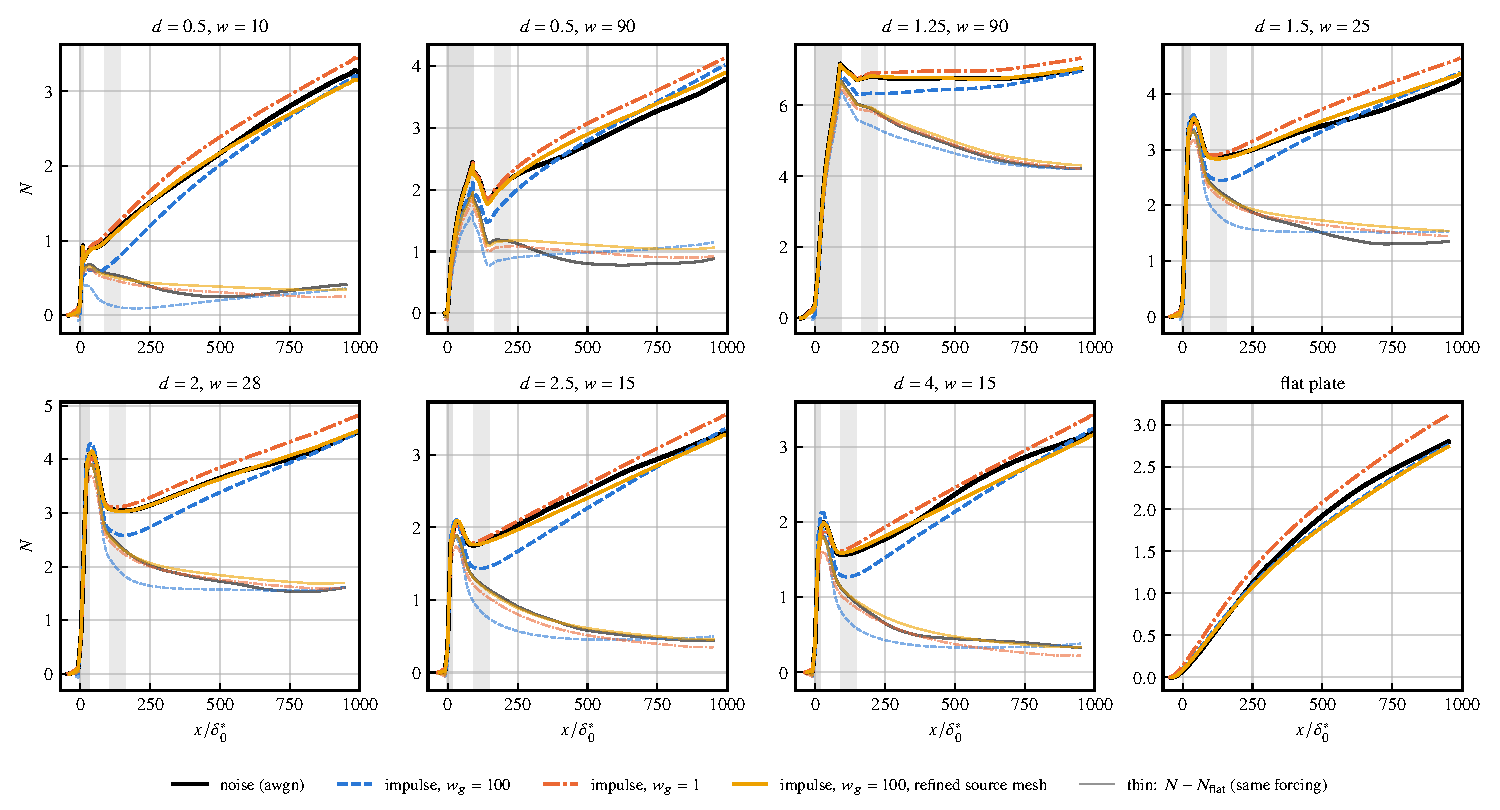
\includegraphics[width=\linewidth,height=0.88\textheight,keepaspectratio]{../../../images/nfactorImpulseVsNoise.pdf}

	\vspace{-0.5cm}
	\begin{itemize}
	  \item $w_g$ is the weight on the gaussian envelope $b$.
	\end{itemize}
	\end{frame}

\end{document}
